% =====================================================================
\section{Supplementary material}\label{app:supp}

\subsection{Bootstrap results by joint regime}\label{app:tables}
\begin{table}[h]
\centering
\caption{Mean paired benefit of history ($E^{\mathrm{GBC}}-E^{\mathrm{GBH}}$, km) by joint speed--turning regime with 95\% drifter-cluster bootstrap intervals ($B=2000$). Source: \texttt{models/history\_gain\_cluster\_bootstrap.csv} (notebook cell 55).}
\label{tab:boot}
\small
\begin{tabular}{@{}llrrrr@{}}
\toprule
Speed & Turning & Cases & Drifters & Mean benefit & 95\% interval \\
\midrule
Low & Low       & \num{946}   & 38 & 2.00 & [1.24, 2.71] \\
Low & Medium    & \num{8263}  & 55 & 2.36 & [1.93, 2.74] \\
Low & High      & \num{15288} & 57 & 2.76 & [2.31, 3.13] \\
Medium & Low    & \num{5225}  & 54 & 3.26 & [2.67, 3.74] \\
Medium & Medium & \num{10394} & 65 & 3.23 & [2.72, 3.68] \\
Medium & High   & \num{8427}  & 59 & 4.65 & [3.86, 5.33] \\
High & Low      & \num{24399} & 65 & 4.11 & [2.94, 5.31] \\
High & Medium   & \num{5775}  & 65 & 3.63 & [2.52, 4.67] \\
High & High     & \num{3816}  & 44 & 7.03 & [5.38, 9.17] \\
\midrule
\multicolumn{2}{@{}l}{All (defined turning)} & \num{82533} & 78 & 3.65 & [3.14, 4.14] \\
\bottomrule
\end{tabular}
\end{table}

\subsection{Reproducibility map}\label{app:repro}
All results come from \texttt{notebook/08\_reoprt\_part\_1.ipynb} (sic), executed top to bottom. The main artefacts are listed below; the report's own figure script is \texttt{report/scripts/make\_figures.py}, which reads only saved outputs.

{\small
\begin{tabularx}{\textwidth}{@{}>{\raggedright\arraybackslash}p{0.38\textwidth}>{\raggedright\arraybackslash}X@{}}
\toprule
Result & Notebook cell(s) and saved artefact \\
\midrule
Cohort, features, split (\cref{tab:cohort,tab:features}) & cells 4--8; \texttt{data/processed/modelling\_dataset\_final.parquet} \\
Baselines, geometric check & cells 9--10, 19, 23, 25 \\
Tuning and validation (\cref{tab:tuning}) & cells 27--36; \texttt{models/*\_validation\_results.csv}, \texttt{final\_validation\_comparison.csv} \\
Test evaluation (\cref{tab:results}, \cref{fig:test}) & cell 39; \texttt{models/final\_test\_comparison.csv}, \texttt{data/processed/report\_test\_predictions.parquet} \\
Motion regimes, joint, bootstrap (\cref{tab:motion}, \cref{fig:motion,fig:joint,fig:boot}) & cells 49--57; \texttt{models/motion\_*.csv}, \texttt{history\_gain\_cluster\_bootstrap.csv} \\
Spatial, temporal, SST (\cref{fig:spatial,fig:temporal,fig:sst}, \cref{tab:temporal,tab:sst}) & cells 60--74; \texttt{data/processed/report\_sst\_ablation\_validation.csv} \\
Figures \ref{fig:region}, \ref{fig:test}, \ref{fig:spatial}; drogue share & \texttt{report/scripts/make\_figures.py} (saved outputs only) \\
\bottomrule
\end{tabularx}}

\subsection{Additional trajectory comparisons}\label{app:figs}
\Cref{fig:family,fig:family2} extend \cref{fig:traj} to the remaining baseline and history-enhanced models.

\begin{figure}[p]
  \centering
  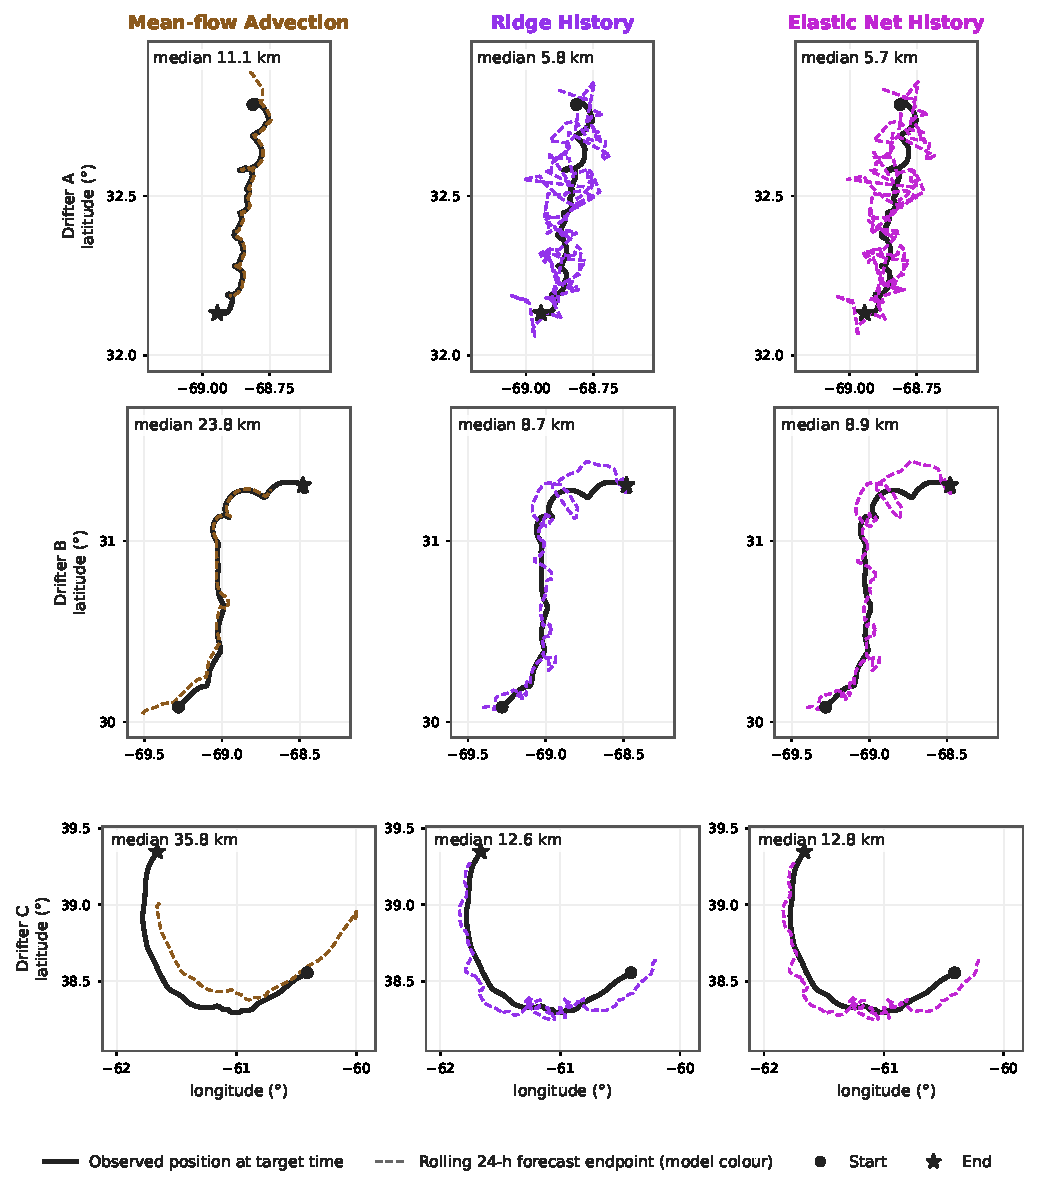
\includegraphics[width=0.86\textwidth]{figures/generated/fig_traj_mf_linear.pdf}
  \caption{Rolling 24-hour forecast endpoints for Mean-flow Advection, Ridge History and Elastic Net History, for the same drifters, windows and axes as \cref{fig:traj}. Ridge and Elastic Net tracks are nearly identical; Mean-flow Advection has much larger errors for drifters B and C (window medians \SI{23.8}{} and \SI{35.8}{km}) than for A (\SI{11.1}{km}). Re-plotted from saved test predictions (notebook cell 46 selection).}
  \label{fig:family}
\end{figure}

\begin{figure}[p]
  \centering
  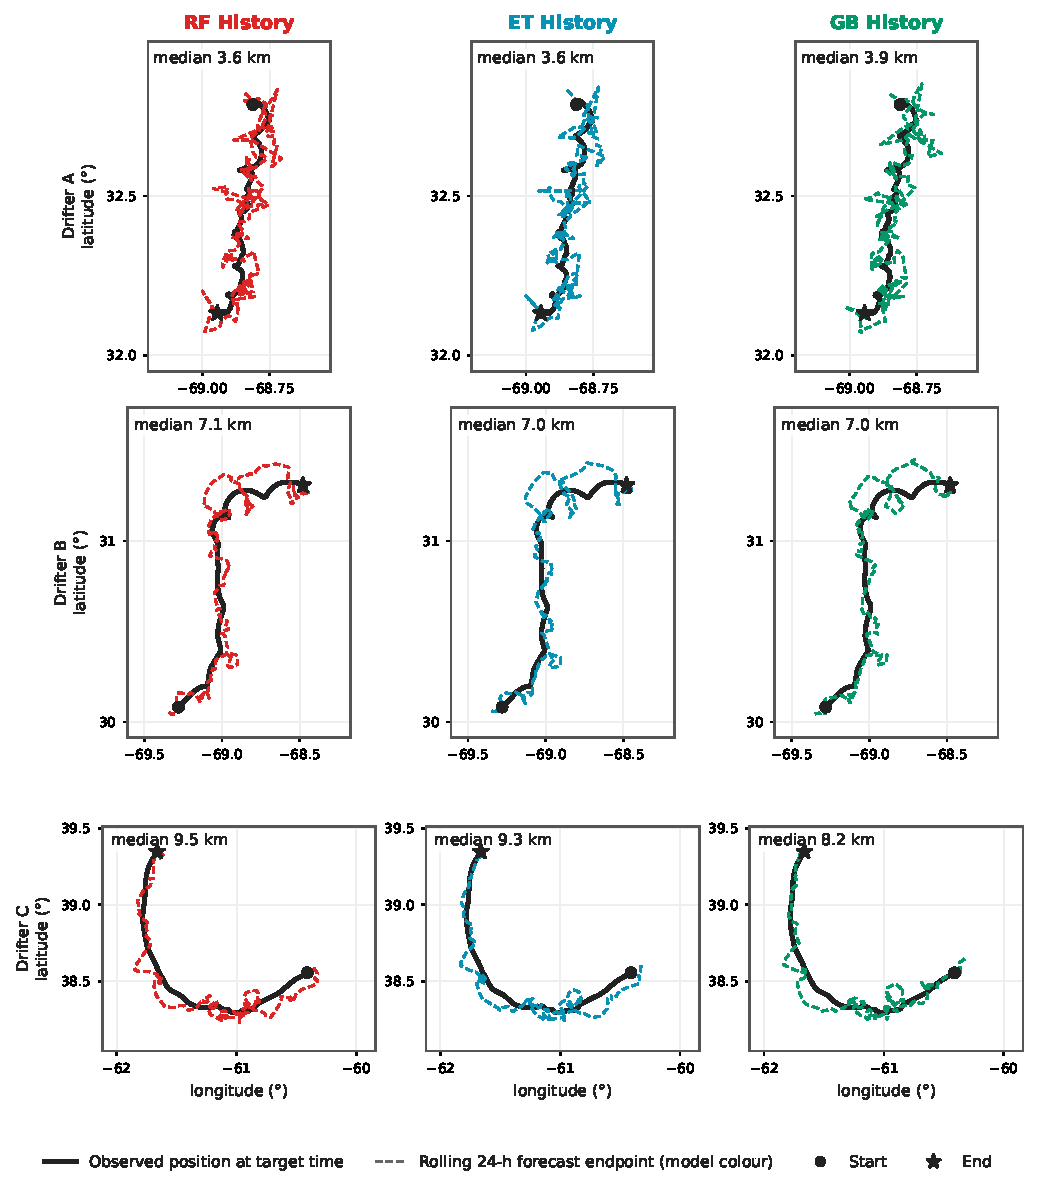
\includegraphics[width=0.86\textwidth]{figures/generated/fig_traj_trees.pdf}
  \caption{As \cref{fig:family} for RF History, ET History and \GBH{}. The three tree ensembles produce visually indistinguishable rolling forecasts, consistent with their near-identical test errors (\cref{tab:results}).}
  \label{fig:family2}
\end{figure}
